
% Default to the notebook output style

    


% Inherit from the specified cell style.




    
\documentclass[11pt]{article}

    
    
    \usepackage[T1]{fontenc}
    % Nicer default font (+ math font) than Computer Modern for most use cases
    \usepackage{mathpazo}

    % Basic figure setup, for now with no caption control since it's done
    % automatically by Pandoc (which extracts ![](path) syntax from Markdown).
    \usepackage{graphicx}
    % We will generate all images so they have a width \maxwidth. This means
    % that they will get their normal width if they fit onto the page, but
    % are scaled down if they would overflow the margins.
    \makeatletter
    \def\maxwidth{\ifdim\Gin@nat@width>\linewidth\linewidth
    \else\Gin@nat@width\fi}
    \makeatother
    \let\Oldincludegraphics\includegraphics
    % Set max figure width to be 80% of text width, for now hardcoded.
    \renewcommand{\includegraphics}[1]{\Oldincludegraphics[width=.8\maxwidth]{#1}}
    % Ensure that by default, figures have no caption (until we provide a
    % proper Figure object with a Caption API and a way to capture that
    % in the conversion process - todo).
    \usepackage{caption}
    \DeclareCaptionLabelFormat{nolabel}{}
    \captionsetup{labelformat=nolabel}

    \usepackage{adjustbox} % Used to constrain images to a maximum size 
    \usepackage{xcolor} % Allow colors to be defined
    \usepackage{enumerate} % Needed for markdown enumerations to work
    \usepackage{geometry} % Used to adjust the document margins
    \usepackage{amsmath} % Equations
    \usepackage{amssymb} % Equations
    \usepackage{textcomp} % defines textquotesingle
    % Hack from http://tex.stackexchange.com/a/47451/13684:
    \AtBeginDocument{%
        \def\PYZsq{\textquotesingle}% Upright quotes in Pygmentized code
    }
    \usepackage{upquote} % Upright quotes for verbatim code
    \usepackage{eurosym} % defines \euro
    \usepackage[mathletters]{ucs} % Extended unicode (utf-8) support
    \usepackage[utf8x]{inputenc} % Allow utf-8 characters in the tex document
    \usepackage{fancyvrb} % verbatim replacement that allows latex
    \usepackage{grffile} % extends the file name processing of package graphics 
                         % to support a larger range 
    % The hyperref package gives us a pdf with properly built
    % internal navigation ('pdf bookmarks' for the table of contents,
    % internal cross-reference links, web links for URLs, etc.)
    \usepackage{hyperref}
    \usepackage{longtable} % longtable support required by pandoc >1.10
    \usepackage{booktabs}  % table support for pandoc > 1.12.2
    \usepackage[inline]{enumitem} % IRkernel/repr support (it uses the enumerate* environment)
    \usepackage[normalem]{ulem} % ulem is needed to support strikethroughs (\sout)
                                % normalem makes italics be italics, not underlines
    

    
    
    % Colors for the hyperref package
    \definecolor{urlcolor}{rgb}{0,.145,.698}
    \definecolor{linkcolor}{rgb}{.71,0.21,0.01}
    \definecolor{citecolor}{rgb}{.12,.54,.11}

    % ANSI colors
    \definecolor{ansi-black}{HTML}{3E424D}
    \definecolor{ansi-black-intense}{HTML}{282C36}
    \definecolor{ansi-red}{HTML}{E75C58}
    \definecolor{ansi-red-intense}{HTML}{B22B31}
    \definecolor{ansi-green}{HTML}{00A250}
    \definecolor{ansi-green-intense}{HTML}{007427}
    \definecolor{ansi-yellow}{HTML}{DDB62B}
    \definecolor{ansi-yellow-intense}{HTML}{B27D12}
    \definecolor{ansi-blue}{HTML}{208FFB}
    \definecolor{ansi-blue-intense}{HTML}{0065CA}
    \definecolor{ansi-magenta}{HTML}{D160C4}
    \definecolor{ansi-magenta-intense}{HTML}{A03196}
    \definecolor{ansi-cyan}{HTML}{60C6C8}
    \definecolor{ansi-cyan-intense}{HTML}{258F8F}
    \definecolor{ansi-white}{HTML}{C5C1B4}
    \definecolor{ansi-white-intense}{HTML}{A1A6B2}

    % commands and environments needed by pandoc snippets
    % extracted from the output of `pandoc -s`
    \providecommand{\tightlist}{%
      \setlength{\itemsep}{0pt}\setlength{\parskip}{0pt}}
    \DefineVerbatimEnvironment{Highlighting}{Verbatim}{commandchars=\\\{\}}
    % Add ',fontsize=\small' for more characters per line
    \newenvironment{Shaded}{}{}
    \newcommand{\KeywordTok}[1]{\textcolor[rgb]{0.00,0.44,0.13}{\textbf{{#1}}}}
    \newcommand{\DataTypeTok}[1]{\textcolor[rgb]{0.56,0.13,0.00}{{#1}}}
    \newcommand{\DecValTok}[1]{\textcolor[rgb]{0.25,0.63,0.44}{{#1}}}
    \newcommand{\BaseNTok}[1]{\textcolor[rgb]{0.25,0.63,0.44}{{#1}}}
    \newcommand{\FloatTok}[1]{\textcolor[rgb]{0.25,0.63,0.44}{{#1}}}
    \newcommand{\CharTok}[1]{\textcolor[rgb]{0.25,0.44,0.63}{{#1}}}
    \newcommand{\StringTok}[1]{\textcolor[rgb]{0.25,0.44,0.63}{{#1}}}
    \newcommand{\CommentTok}[1]{\textcolor[rgb]{0.38,0.63,0.69}{\textit{{#1}}}}
    \newcommand{\OtherTok}[1]{\textcolor[rgb]{0.00,0.44,0.13}{{#1}}}
    \newcommand{\AlertTok}[1]{\textcolor[rgb]{1.00,0.00,0.00}{\textbf{{#1}}}}
    \newcommand{\FunctionTok}[1]{\textcolor[rgb]{0.02,0.16,0.49}{{#1}}}
    \newcommand{\RegionMarkerTok}[1]{{#1}}
    \newcommand{\ErrorTok}[1]{\textcolor[rgb]{1.00,0.00,0.00}{\textbf{{#1}}}}
    \newcommand{\NormalTok}[1]{{#1}}
    
    % Additional commands for more recent versions of Pandoc
    \newcommand{\ConstantTok}[1]{\textcolor[rgb]{0.53,0.00,0.00}{{#1}}}
    \newcommand{\SpecialCharTok}[1]{\textcolor[rgb]{0.25,0.44,0.63}{{#1}}}
    \newcommand{\VerbatimStringTok}[1]{\textcolor[rgb]{0.25,0.44,0.63}{{#1}}}
    \newcommand{\SpecialStringTok}[1]{\textcolor[rgb]{0.73,0.40,0.53}{{#1}}}
    \newcommand{\ImportTok}[1]{{#1}}
    \newcommand{\DocumentationTok}[1]{\textcolor[rgb]{0.73,0.13,0.13}{\textit{{#1}}}}
    \newcommand{\AnnotationTok}[1]{\textcolor[rgb]{0.38,0.63,0.69}{\textbf{\textit{{#1}}}}}
    \newcommand{\CommentVarTok}[1]{\textcolor[rgb]{0.38,0.63,0.69}{\textbf{\textit{{#1}}}}}
    \newcommand{\VariableTok}[1]{\textcolor[rgb]{0.10,0.09,0.49}{{#1}}}
    \newcommand{\ControlFlowTok}[1]{\textcolor[rgb]{0.00,0.44,0.13}{\textbf{{#1}}}}
    \newcommand{\OperatorTok}[1]{\textcolor[rgb]{0.40,0.40,0.40}{{#1}}}
    \newcommand{\BuiltInTok}[1]{{#1}}
    \newcommand{\ExtensionTok}[1]{{#1}}
    \newcommand{\PreprocessorTok}[1]{\textcolor[rgb]{0.74,0.48,0.00}{{#1}}}
    \newcommand{\AttributeTok}[1]{\textcolor[rgb]{0.49,0.56,0.16}{{#1}}}
    \newcommand{\InformationTok}[1]{\textcolor[rgb]{0.38,0.63,0.69}{\textbf{\textit{{#1}}}}}
    \newcommand{\WarningTok}[1]{\textcolor[rgb]{0.38,0.63,0.69}{\textbf{\textit{{#1}}}}}
    
    
    % Define a nice break command that doesn't care if a line doesn't already
    % exist.
    \def\br{\hspace*{\fill} \\* }
    % Math Jax compatability definitions
    \def\gt{>}
    \def\lt{<}
    % Document parameters
    \title{tutorial\_P1\_TeensyPythonWalkthrough}
    
    
    

    % Pygments definitions
    
\makeatletter
\def\PY@reset{\let\PY@it=\relax \let\PY@bf=\relax%
    \let\PY@ul=\relax \let\PY@tc=\relax%
    \let\PY@bc=\relax \let\PY@ff=\relax}
\def\PY@tok#1{\csname PY@tok@#1\endcsname}
\def\PY@toks#1+{\ifx\relax#1\empty\else%
    \PY@tok{#1}\expandafter\PY@toks\fi}
\def\PY@do#1{\PY@bc{\PY@tc{\PY@ul{%
    \PY@it{\PY@bf{\PY@ff{#1}}}}}}}
\def\PY#1#2{\PY@reset\PY@toks#1+\relax+\PY@do{#2}}

\expandafter\def\csname PY@tok@w\endcsname{\def\PY@tc##1{\textcolor[rgb]{0.73,0.73,0.73}{##1}}}
\expandafter\def\csname PY@tok@c\endcsname{\let\PY@it=\textit\def\PY@tc##1{\textcolor[rgb]{0.25,0.50,0.50}{##1}}}
\expandafter\def\csname PY@tok@cp\endcsname{\def\PY@tc##1{\textcolor[rgb]{0.74,0.48,0.00}{##1}}}
\expandafter\def\csname PY@tok@k\endcsname{\let\PY@bf=\textbf\def\PY@tc##1{\textcolor[rgb]{0.00,0.50,0.00}{##1}}}
\expandafter\def\csname PY@tok@kp\endcsname{\def\PY@tc##1{\textcolor[rgb]{0.00,0.50,0.00}{##1}}}
\expandafter\def\csname PY@tok@kt\endcsname{\def\PY@tc##1{\textcolor[rgb]{0.69,0.00,0.25}{##1}}}
\expandafter\def\csname PY@tok@o\endcsname{\def\PY@tc##1{\textcolor[rgb]{0.40,0.40,0.40}{##1}}}
\expandafter\def\csname PY@tok@ow\endcsname{\let\PY@bf=\textbf\def\PY@tc##1{\textcolor[rgb]{0.67,0.13,1.00}{##1}}}
\expandafter\def\csname PY@tok@nb\endcsname{\def\PY@tc##1{\textcolor[rgb]{0.00,0.50,0.00}{##1}}}
\expandafter\def\csname PY@tok@nf\endcsname{\def\PY@tc##1{\textcolor[rgb]{0.00,0.00,1.00}{##1}}}
\expandafter\def\csname PY@tok@nc\endcsname{\let\PY@bf=\textbf\def\PY@tc##1{\textcolor[rgb]{0.00,0.00,1.00}{##1}}}
\expandafter\def\csname PY@tok@nn\endcsname{\let\PY@bf=\textbf\def\PY@tc##1{\textcolor[rgb]{0.00,0.00,1.00}{##1}}}
\expandafter\def\csname PY@tok@ne\endcsname{\let\PY@bf=\textbf\def\PY@tc##1{\textcolor[rgb]{0.82,0.25,0.23}{##1}}}
\expandafter\def\csname PY@tok@nv\endcsname{\def\PY@tc##1{\textcolor[rgb]{0.10,0.09,0.49}{##1}}}
\expandafter\def\csname PY@tok@no\endcsname{\def\PY@tc##1{\textcolor[rgb]{0.53,0.00,0.00}{##1}}}
\expandafter\def\csname PY@tok@nl\endcsname{\def\PY@tc##1{\textcolor[rgb]{0.63,0.63,0.00}{##1}}}
\expandafter\def\csname PY@tok@ni\endcsname{\let\PY@bf=\textbf\def\PY@tc##1{\textcolor[rgb]{0.60,0.60,0.60}{##1}}}
\expandafter\def\csname PY@tok@na\endcsname{\def\PY@tc##1{\textcolor[rgb]{0.49,0.56,0.16}{##1}}}
\expandafter\def\csname PY@tok@nt\endcsname{\let\PY@bf=\textbf\def\PY@tc##1{\textcolor[rgb]{0.00,0.50,0.00}{##1}}}
\expandafter\def\csname PY@tok@nd\endcsname{\def\PY@tc##1{\textcolor[rgb]{0.67,0.13,1.00}{##1}}}
\expandafter\def\csname PY@tok@s\endcsname{\def\PY@tc##1{\textcolor[rgb]{0.73,0.13,0.13}{##1}}}
\expandafter\def\csname PY@tok@sd\endcsname{\let\PY@it=\textit\def\PY@tc##1{\textcolor[rgb]{0.73,0.13,0.13}{##1}}}
\expandafter\def\csname PY@tok@si\endcsname{\let\PY@bf=\textbf\def\PY@tc##1{\textcolor[rgb]{0.73,0.40,0.53}{##1}}}
\expandafter\def\csname PY@tok@se\endcsname{\let\PY@bf=\textbf\def\PY@tc##1{\textcolor[rgb]{0.73,0.40,0.13}{##1}}}
\expandafter\def\csname PY@tok@sr\endcsname{\def\PY@tc##1{\textcolor[rgb]{0.73,0.40,0.53}{##1}}}
\expandafter\def\csname PY@tok@ss\endcsname{\def\PY@tc##1{\textcolor[rgb]{0.10,0.09,0.49}{##1}}}
\expandafter\def\csname PY@tok@sx\endcsname{\def\PY@tc##1{\textcolor[rgb]{0.00,0.50,0.00}{##1}}}
\expandafter\def\csname PY@tok@m\endcsname{\def\PY@tc##1{\textcolor[rgb]{0.40,0.40,0.40}{##1}}}
\expandafter\def\csname PY@tok@gh\endcsname{\let\PY@bf=\textbf\def\PY@tc##1{\textcolor[rgb]{0.00,0.00,0.50}{##1}}}
\expandafter\def\csname PY@tok@gu\endcsname{\let\PY@bf=\textbf\def\PY@tc##1{\textcolor[rgb]{0.50,0.00,0.50}{##1}}}
\expandafter\def\csname PY@tok@gd\endcsname{\def\PY@tc##1{\textcolor[rgb]{0.63,0.00,0.00}{##1}}}
\expandafter\def\csname PY@tok@gi\endcsname{\def\PY@tc##1{\textcolor[rgb]{0.00,0.63,0.00}{##1}}}
\expandafter\def\csname PY@tok@gr\endcsname{\def\PY@tc##1{\textcolor[rgb]{1.00,0.00,0.00}{##1}}}
\expandafter\def\csname PY@tok@ge\endcsname{\let\PY@it=\textit}
\expandafter\def\csname PY@tok@gs\endcsname{\let\PY@bf=\textbf}
\expandafter\def\csname PY@tok@gp\endcsname{\let\PY@bf=\textbf\def\PY@tc##1{\textcolor[rgb]{0.00,0.00,0.50}{##1}}}
\expandafter\def\csname PY@tok@go\endcsname{\def\PY@tc##1{\textcolor[rgb]{0.53,0.53,0.53}{##1}}}
\expandafter\def\csname PY@tok@gt\endcsname{\def\PY@tc##1{\textcolor[rgb]{0.00,0.27,0.87}{##1}}}
\expandafter\def\csname PY@tok@err\endcsname{\def\PY@bc##1{\setlength{\fboxsep}{0pt}\fcolorbox[rgb]{1.00,0.00,0.00}{1,1,1}{\strut ##1}}}
\expandafter\def\csname PY@tok@kc\endcsname{\let\PY@bf=\textbf\def\PY@tc##1{\textcolor[rgb]{0.00,0.50,0.00}{##1}}}
\expandafter\def\csname PY@tok@kd\endcsname{\let\PY@bf=\textbf\def\PY@tc##1{\textcolor[rgb]{0.00,0.50,0.00}{##1}}}
\expandafter\def\csname PY@tok@kn\endcsname{\let\PY@bf=\textbf\def\PY@tc##1{\textcolor[rgb]{0.00,0.50,0.00}{##1}}}
\expandafter\def\csname PY@tok@kr\endcsname{\let\PY@bf=\textbf\def\PY@tc##1{\textcolor[rgb]{0.00,0.50,0.00}{##1}}}
\expandafter\def\csname PY@tok@bp\endcsname{\def\PY@tc##1{\textcolor[rgb]{0.00,0.50,0.00}{##1}}}
\expandafter\def\csname PY@tok@fm\endcsname{\def\PY@tc##1{\textcolor[rgb]{0.00,0.00,1.00}{##1}}}
\expandafter\def\csname PY@tok@vc\endcsname{\def\PY@tc##1{\textcolor[rgb]{0.10,0.09,0.49}{##1}}}
\expandafter\def\csname PY@tok@vg\endcsname{\def\PY@tc##1{\textcolor[rgb]{0.10,0.09,0.49}{##1}}}
\expandafter\def\csname PY@tok@vi\endcsname{\def\PY@tc##1{\textcolor[rgb]{0.10,0.09,0.49}{##1}}}
\expandafter\def\csname PY@tok@vm\endcsname{\def\PY@tc##1{\textcolor[rgb]{0.10,0.09,0.49}{##1}}}
\expandafter\def\csname PY@tok@sa\endcsname{\def\PY@tc##1{\textcolor[rgb]{0.73,0.13,0.13}{##1}}}
\expandafter\def\csname PY@tok@sb\endcsname{\def\PY@tc##1{\textcolor[rgb]{0.73,0.13,0.13}{##1}}}
\expandafter\def\csname PY@tok@sc\endcsname{\def\PY@tc##1{\textcolor[rgb]{0.73,0.13,0.13}{##1}}}
\expandafter\def\csname PY@tok@dl\endcsname{\def\PY@tc##1{\textcolor[rgb]{0.73,0.13,0.13}{##1}}}
\expandafter\def\csname PY@tok@s2\endcsname{\def\PY@tc##1{\textcolor[rgb]{0.73,0.13,0.13}{##1}}}
\expandafter\def\csname PY@tok@sh\endcsname{\def\PY@tc##1{\textcolor[rgb]{0.73,0.13,0.13}{##1}}}
\expandafter\def\csname PY@tok@s1\endcsname{\def\PY@tc##1{\textcolor[rgb]{0.73,0.13,0.13}{##1}}}
\expandafter\def\csname PY@tok@mb\endcsname{\def\PY@tc##1{\textcolor[rgb]{0.40,0.40,0.40}{##1}}}
\expandafter\def\csname PY@tok@mf\endcsname{\def\PY@tc##1{\textcolor[rgb]{0.40,0.40,0.40}{##1}}}
\expandafter\def\csname PY@tok@mh\endcsname{\def\PY@tc##1{\textcolor[rgb]{0.40,0.40,0.40}{##1}}}
\expandafter\def\csname PY@tok@mi\endcsname{\def\PY@tc##1{\textcolor[rgb]{0.40,0.40,0.40}{##1}}}
\expandafter\def\csname PY@tok@il\endcsname{\def\PY@tc##1{\textcolor[rgb]{0.40,0.40,0.40}{##1}}}
\expandafter\def\csname PY@tok@mo\endcsname{\def\PY@tc##1{\textcolor[rgb]{0.40,0.40,0.40}{##1}}}
\expandafter\def\csname PY@tok@ch\endcsname{\let\PY@it=\textit\def\PY@tc##1{\textcolor[rgb]{0.25,0.50,0.50}{##1}}}
\expandafter\def\csname PY@tok@cm\endcsname{\let\PY@it=\textit\def\PY@tc##1{\textcolor[rgb]{0.25,0.50,0.50}{##1}}}
\expandafter\def\csname PY@tok@cpf\endcsname{\let\PY@it=\textit\def\PY@tc##1{\textcolor[rgb]{0.25,0.50,0.50}{##1}}}
\expandafter\def\csname PY@tok@c1\endcsname{\let\PY@it=\textit\def\PY@tc##1{\textcolor[rgb]{0.25,0.50,0.50}{##1}}}
\expandafter\def\csname PY@tok@cs\endcsname{\let\PY@it=\textit\def\PY@tc##1{\textcolor[rgb]{0.25,0.50,0.50}{##1}}}

\def\PYZbs{\char`\\}
\def\PYZus{\char`\_}
\def\PYZob{\char`\{}
\def\PYZcb{\char`\}}
\def\PYZca{\char`\^}
\def\PYZam{\char`\&}
\def\PYZlt{\char`\<}
\def\PYZgt{\char`\>}
\def\PYZsh{\char`\#}
\def\PYZpc{\char`\%}
\def\PYZdl{\char`\$}
\def\PYZhy{\char`\-}
\def\PYZsq{\char`\'}
\def\PYZdq{\char`\"}
\def\PYZti{\char`\~}
% for compatibility with earlier versions
\def\PYZat{@}
\def\PYZlb{[}
\def\PYZrb{]}
\makeatother


    % Exact colors from NB
    \definecolor{incolor}{rgb}{0.0, 0.0, 0.5}
    \definecolor{outcolor}{rgb}{0.545, 0.0, 0.0}



    
    % Prevent overflowing lines due to hard-to-break entities
    \sloppy 
    % Setup hyperref package
    \hypersetup{
      breaklinks=true,  % so long urls are correctly broken across lines
      colorlinks=true,
      urlcolor=urlcolor,
      linkcolor=linkcolor,
      citecolor=citecolor,
      }
    % Slightly bigger margins than the latex defaults
    
    \geometry{verbose,tmargin=1in,bmargin=1in,lmargin=1in,rmargin=1in}
    
    

    \begin{document}
    
    
    \maketitle
    
    

    
    \section{Implementing a Detection
Trial}\label{implementing-a-detection-trial}

    \subsection{Here is our state scheme:}\label{here-is-our-state-scheme}

\begin{figure}
\centering
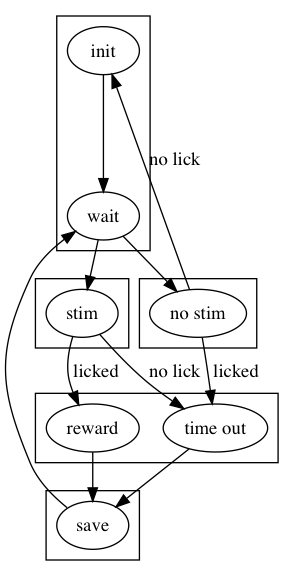
\includegraphics{https://raw.githubusercontent.com/cdeister/csVisual/master/stateGraphs/detectionStates.png}
\caption{Detection}
\end{figure}

    \href{https://github.com/cdeister/csVisual/tree/master/microcontrollerCode/csVisual_DetectionStates}{This
code needs to be on a teensy}

    \section{This is part 1. Some basics. We will connect to a serial
object, change states, read some data over serial, plot that data, read
more and detect 'licks.' You should understand how to parse serial data
with ease after
this.}\label{this-is-part-1.-some-basics.-we-will-connect-to-a-serial-object-change-states-read-some-data-over-serial-plot-that-data-read-more-and-detect-licks.-you-should-understand-how-to-parse-serial-data-with-ease-after-this.}

    \begin{Verbatim}[commandchars=\\\{\}]
{\color{incolor}In [{\color{incolor}1}]:} \PY{k+kn}{import} \PY{n+nn}{warnings}
        \PY{n}{warnings}\PY{o}{.}\PY{n}{filterwarnings}\PY{p}{(}\PY{l+s+s1}{\PYZsq{}}\PY{l+s+s1}{ignore}\PY{l+s+s1}{\PYZsq{}}\PY{p}{)}
        
        \PY{k+kn}{import} \PY{n+nn}{serial}
        \PY{k+kn}{import} \PY{n+nn}{numpy} \PY{k}{as} \PY{n+nn}{np}
        \PY{o}{\PYZpc{}}\PY{k}{matplotlib} notebook
        \PY{c+c1}{\PYZsh{} Inline is jank, but you have to hand code fig nums.}
        \PY{k+kn}{import} \PY{n+nn}{matplotlib}\PY{n+nn}{.}\PY{n+nn}{pyplot} \PY{k}{as} \PY{n+nn}{plt}
        \PY{k+kn}{import} \PY{n+nn}{h5py}
        \PY{k+kn}{import} \PY{n+nn}{os}
        \PY{k+kn}{import} \PY{n+nn}{datetime}
        \PY{k+kn}{import} \PY{n+nn}{time}
\end{Verbatim}


    \begin{Verbatim}[commandchars=\\\{\}]
{\color{incolor}In [{\color{incolor}2}]:} \PY{c+c1}{\PYZsh{} first connect to the teensy}
        
        \PY{k}{def} \PY{n+nf}{connectTeensy}\PY{p}{(}\PY{p}{)}\PY{p}{:}
            \PY{n}{baudRate}\PY{o}{=}\PY{l+m+mi}{115200}
            \PY{n}{teensyPath}\PY{o}{=}\PY{l+s+s1}{\PYZsq{}}\PY{l+s+s1}{/dev/cu.usbmodem2762721}\PY{l+s+s1}{\PYZsq{}}
            \PY{n}{teensy} \PY{o}{=} \PY{n}{serial}\PY{o}{.}\PY{n}{Serial}\PY{p}{(}\PY{n}{teensyPath}\PY{p}{,}\PY{n}{baudRate}\PY{p}{)}
            \PY{k}{return} \PY{n}{teensy}
\end{Verbatim}


    \begin{Verbatim}[commandchars=\\\{\}]
{\color{incolor}In [{\color{incolor}3}]:} \PY{k}{try}\PY{p}{:}
            \PY{n}{vTeensy}\PY{o}{=}\PY{n}{connectTeensy}\PY{p}{(}\PY{p}{)}
            \PY{n+nb}{print}\PY{p}{(}\PY{l+s+s2}{\PYZdq{}}\PY{l+s+s2}{connected!}\PY{l+s+s2}{\PYZdq{}}\PY{p}{)}
        \PY{k}{except}\PY{p}{:}
            \PY{n+nb}{print}\PY{p}{(}\PY{l+s+s2}{\PYZdq{}}\PY{l+s+s2}{couldn}\PY{l+s+s2}{\PYZsq{}}\PY{l+s+s2}{t connect; check the teensy}\PY{l+s+s2}{\PYZdq{}}\PY{p}{)}
\end{Verbatim}


    \begin{Verbatim}[commandchars=\\\{\}]
connected!

    \end{Verbatim}

    \textbf{For this first part, I assume you know very little about python
and have not parsed my code at all. Therefore, we will reinforce key
first principles. Next chapter, we will get back to a trial in a task.}

** Please scroll through the notebook to get a sense of what is coming**

    \begin{Verbatim}[commandchars=\\\{\}]
{\color{incolor}In [{\color{incolor}4}]:} \PY{c+c1}{\PYZsh{} First ask the teensy what state it is in. Ignore the output if it isnt a warning etc.}
        \PY{n}{vTeensy}\PY{o}{.}\PY{n}{write}\PY{p}{(}\PY{l+s+s1}{\PYZsq{}}\PY{l+s+s1}{a\PYZlt{}}\PY{l+s+s1}{\PYZsq{}}\PY{o}{.}\PY{n}{encode}\PY{p}{(}\PY{l+s+s1}{\PYZsq{}}\PY{l+s+s1}{utf\PYZhy{}8}\PY{l+s+s1}{\PYZsq{}}\PY{p}{)}\PY{p}{)}
\end{Verbatim}


\begin{Verbatim}[commandchars=\\\{\}]
{\color{outcolor}Out[{\color{outcolor}4}]:} 2
\end{Verbatim}
            
    \begin{Verbatim}[commandchars=\\\{\}]
{\color{incolor}In [{\color{incolor}5}]:} \PY{c+c1}{\PYZsh{} We should get an \PYZsq{}echo\PYZsq{} line back in the buffer. Assuming the teensy is in state 0 it won\PYZsq{}t send anything}
        \PY{c+c1}{\PYZsh{} else, so only one line should be in the serial buffer now. Let\PYZsq{}s grab it and store it in a variable named sR.}
        \PY{n}{sR}\PY{o}{=}\PY{n}{vTeensy}\PY{o}{.}\PY{n}{readline}\PY{p}{(}\PY{p}{)}\PY{o}{.}\PY{n}{strip}\PY{p}{(}\PY{p}{)}\PY{o}{.}\PY{n}{decode}\PY{p}{(}\PY{p}{)}
        \PY{c+c1}{\PYZsh{} You can look at pySerial\PYZsq{}s documentation to see what strip and decode do, it\PYZsq{}s not a bad idea.}
        \PY{c+c1}{\PYZsh{} http://pyserial.readthedocs.io/en/latest/pyserial\PYZus{}api.html}
\end{Verbatim}


    \begin{Verbatim}[commandchars=\\\{\}]
{\color{incolor}In [{\color{incolor}6}]:} \PY{c+c1}{\PYZsh{} Let\PYZsq{}s see what we got:}
        \PY{n+nb}{print}\PY{p}{(}\PY{n}{sR}\PY{p}{)}
\end{Verbatim}


    \begin{Verbatim}[commandchars=\\\{\}]
echo,0,0,\textasciitilde{}

    \end{Verbatim}

    \paragraph{You should see
"echo,0,0,\textasciitilde{}"}\label{you-should-see-echo00}

\subparagraph{What is going on here, is I set the teensy code to echo
back the state of a variable it tracks with the various headers
available. 'a' is the header for the state variable. It happens to be
element 0 of the array that tracks them. And, we expect it to be in
state 0. The line is in the form
of:}\label{what-is-going-on-here-is-i-set-the-teensy-code-to-echo-back-the-state-of-a-variable-it-tracks-with-the-various-headers-available.-a-is-the-header-for-the-state-variable.-it-happens-to-be-element-0-of-the-array-that-tracks-them.-and-we-expect-it-to-be-in-state-0.-the-line-is-in-the-form-of}

echo,varIndex,varValue,\textasciitilde{} \#\#\#\#\# Where echo and
\textasciitilde{} are always present and can help parse the line as you
have a header and closer.

    \begin{Verbatim}[commandchars=\\\{\}]
{\color{incolor}In [{\color{incolor}7}]:} \PY{n}{splitSR}\PY{o}{=}\PY{n}{sR}\PY{o}{.}\PY{n}{split}\PY{p}{(}\PY{l+s+s1}{\PYZsq{}}\PY{l+s+s1}{,}\PY{l+s+s1}{\PYZsq{}}\PY{p}{)}
\end{Verbatim}


    \begin{Verbatim}[commandchars=\\\{\}]
{\color{incolor}In [{\color{incolor}8}]:} \PY{c+c1}{\PYZsh{} Now we can set up a conditional change to a different state.}
        
        \PY{c+c1}{\PYZsh{} First split sR on commas. Split is a property of all strings. sR is a string.}
        \PY{n+nb}{print}\PY{p}{(}\PY{l+s+s1}{\PYZsq{}}\PY{l+s+s1}{I am showing you that the type of sR is in fact a: }\PY{l+s+si}{\PYZob{}\PYZcb{}}\PY{l+s+s1}{\PYZsq{}}\PY{o}{.}\PY{n}{format}\PY{p}{(}\PY{n+nb}{type}\PY{p}{(}\PY{n}{sR}\PY{p}{)}\PY{p}{)}\PY{p}{)}
        \PY{n}{splitSR}\PY{o}{=}\PY{n}{sR}\PY{o}{.}\PY{n}{split}\PY{p}{(}\PY{l+s+s1}{\PYZsq{}}\PY{l+s+s1}{,}\PY{l+s+s1}{\PYZsq{}}\PY{p}{)}
        
        \PY{k}{if} \PY{n+nb}{int}\PY{p}{(}\PY{n}{splitSR}\PY{p}{[}\PY{l+m+mi}{1}\PY{p}{]}\PY{p}{)}\PY{o}{==}\PY{l+m+mi}{0}\PY{p}{:}
            \PY{c+c1}{\PYZsh{} Then we have a state variable echoed.}
            \PY{k}{if} \PY{n+nb}{int}\PY{p}{(}\PY{n}{splitSR}\PY{p}{[}\PY{l+m+mi}{2}\PY{p}{]}\PY{p}{)}\PY{o}{==}\PY{l+m+mi}{0}\PY{p}{:}
                \PY{n}{vTeensy}\PY{o}{.}\PY{n}{write}\PY{p}{(}\PY{l+s+s1}{\PYZsq{}}\PY{l+s+s1}{a1\PYZgt{}}\PY{l+s+s1}{\PYZsq{}}\PY{o}{.}\PY{n}{encode}\PY{p}{(}\PY{l+s+s1}{\PYZsq{}}\PY{l+s+s1}{utf\PYZhy{}8}\PY{l+s+s1}{\PYZsq{}}\PY{p}{)}\PY{p}{)}
                \PY{n}{time}\PY{o}{.}\PY{n}{sleep}\PY{p}{(}\PY{l+m+mf}{0.05}\PY{p}{)}
                \PY{n}{vTeensy}\PY{o}{.}\PY{n}{write}\PY{p}{(}\PY{l+s+s1}{\PYZsq{}}\PY{l+s+s1}{a0\PYZgt{}}\PY{l+s+s1}{\PYZsq{}}\PY{o}{.}\PY{n}{encode}\PY{p}{(}\PY{l+s+s1}{\PYZsq{}}\PY{l+s+s1}{utf\PYZhy{}8}\PY{l+s+s1}{\PYZsq{}}\PY{p}{)}\PY{p}{)}
                
                
\end{Verbatim}


    \begin{Verbatim}[commandchars=\\\{\}]
I am showing you that the type of sR is in fact a: <class 'str'>

    \end{Verbatim}

    The reason I paused and flipped back to s0 is because s1 dumped a ton of
data onto the buffer that we were not ready for. We slept (paused) for
50 ms, which is PC timed not teensy timed, so we will be off at least a
couple of ms. So we can estimate we should have \textasciitilde{}50
lines in the buffer.

    \begin{Verbatim}[commandchars=\\\{\}]
{\color{incolor}In [{\color{incolor}9}]:} \PY{c+c1}{\PYZsh{} Let\PYZsq{}s get one of the s1 lines.}
        \PY{k}{if} \PY{n}{vTeensy}\PY{o}{.}\PY{n}{inWaiting}\PY{p}{(}\PY{p}{)}\PY{o}{\PYZgt{}}\PY{l+m+mi}{0}\PY{p}{:}
            \PY{n}{sR}\PY{o}{=}\PY{n}{vTeensy}\PY{o}{.}\PY{n}{readline}\PY{p}{(}\PY{p}{)}\PY{o}{.}\PY{n}{strip}\PY{p}{(}\PY{p}{)}\PY{o}{.}\PY{n}{decode}\PY{p}{(}\PY{p}{)}
            \PY{n+nb}{print}\PY{p}{(}\PY{n}{sR}\PY{p}{)}
        \PY{k}{elif} \PY{n}{vTeensy}\PY{o}{.}\PY{n}{inWaiting}\PY{p}{(}\PY{p}{)}\PY{o}{==}\PY{l+m+mi}{0}\PY{p}{:}
            \PY{n+nb}{print}\PY{p}{(}\PY{l+s+s1}{\PYZsq{}}\PY{l+s+s1}{nothing in buffer; teensy ok?}\PY{l+s+s1}{\PYZsq{}}\PY{p}{)}
\end{Verbatim}


    \begin{Verbatim}[commandchars=\\\{\}]
tData,0,0,0,1,1,503

    \end{Verbatim}

    \paragraph{You should see "tData,0,0,0,1,1,XXX" Or something like
that.}\label{you-should-see-tdata00011xxx-or-something-like-that.}

\subparagraph{In all states but 0 the teensy streams a data report line
once a millisecond. It is currently of the
form:}\label{in-all-states-but-0-the-teensy-streams-a-data-report-line-once-a-millisecond.-it-is-currently-of-the-form}

tData,interruptCount,trialTimeInMs,stateTimeInMs,currentStateTeensyThinksItIsIn,analogLickPinAVal,analogLickPinBVal
\#\#\#\# The tData is always in a data report line and it is the main
thing we filter on. The number of variables does not change and can be
used to filter good lines from bad ones too.I want to point out the
three timing variables. \#\#\#\#\# interruptCount is the number of loops
the teensy has done since leaving s0. Because we are using an interrupt
to time the task this should be identical to trial time unless you
change the sample rate and then it will be off by a scalar. Currently
the sample rate is set to 1000 interrupts per second. trialTimeInMs is
time since s0 in ms based on the teensy millis() call. You should have a
constant dt and that dt should be the same as the interrupt dt, if the
funciton fails to return in a ms you will see it reflected here.
stateTimeInMs is unecessary but here for convinence. I offset a timer
when you enter states on the teensy and it counts up from the header on.

    There is still a lot of data in the buffer. Lets see how we did as far
as time being ordered right as we clear out the buffer. We first write a
function to parse lines by headers and variable count, and have it
report if there is new data or not. We can then read itterativley until
this returns a 0 for new data.

    \begin{Verbatim}[commandchars=\\\{\}]
{\color{incolor}In [{\color{incolor}10}]:} \PY{k}{def} \PY{n+nf}{readSerialData}\PY{p}{(}\PY{n}{comObj}\PY{p}{,}\PY{n}{headerString}\PY{p}{,}\PY{n}{varCount}\PY{p}{)}\PY{p}{:}
             \PY{k}{try}\PY{p}{:}
                 \PY{n}{sR}\PY{o}{=}\PY{p}{[}\PY{p}{]}
                 \PY{n}{newData}\PY{o}{=}\PY{l+m+mi}{0}
                 \PY{k}{if} \PY{n}{comObj}\PY{o}{.}\PY{n}{inWaiting}\PY{p}{(}\PY{p}{)}\PY{o}{\PYZgt{}}\PY{l+m+mi}{0}\PY{p}{:}
                     \PY{n}{sR}\PY{o}{=}\PY{n}{comObj}\PY{o}{.}\PY{n}{readline}\PY{p}{(}\PY{p}{)}\PY{o}{.}\PY{n}{strip}\PY{p}{(}\PY{p}{)}\PY{o}{.}\PY{n}{decode}\PY{p}{(}\PY{p}{)}
                     \PY{n}{sR}\PY{o}{=}\PY{n}{sR}\PY{o}{.}\PY{n}{split}\PY{p}{(}\PY{l+s+s1}{\PYZsq{}}\PY{l+s+s1}{,}\PY{l+s+s1}{\PYZsq{}}\PY{p}{)}
                     \PY{k}{if} \PY{n+nb}{len}\PY{p}{(}\PY{n}{sR}\PY{p}{)}\PY{o}{==}\PY{n}{varCount} \PY{o+ow}{and} \PY{n}{sR}\PY{p}{[}\PY{l+m+mi}{0}\PY{p}{]}\PY{o}{==}\PY{n}{headerString}\PY{p}{:}
                         \PY{n}{newData}\PY{o}{=}\PY{l+m+mi}{1}
             \PY{k}{except}\PY{p}{:}
                 \PY{n+nb}{print}\PY{p}{(}\PY{l+s+s1}{\PYZsq{}}\PY{l+s+s1}{read empty}\PY{l+s+s1}{\PYZsq{}}\PY{p}{)}
                 \PY{n}{newData}\PY{o}{=}\PY{l+m+mi}{0}
                 \PY{n}{sR}\PY{o}{=}\PY{p}{[}\PY{p}{]}
                 
             \PY{k}{return} \PY{n}{sR}\PY{p}{,}\PY{n}{newData}
\end{Verbatim}


    \begin{Verbatim}[commandchars=\\\{\}]
{\color{incolor}In [{\color{incolor}11}]:} \PY{c+c1}{\PYZsh{} Let\PYZsq{}s do one line for pedagogy. We should get interrupt \PYZsh{}1  (0  is the first).}
         \PY{p}{[}\PY{n}{curDataLine}\PY{p}{,}\PY{n}{dataAvail}\PY{p}{]}\PY{o}{=}\PY{n}{readSerialData}\PY{p}{(}\PY{n}{vTeensy}\PY{p}{,}\PY{l+s+s1}{\PYZsq{}}\PY{l+s+s1}{tData}\PY{l+s+s1}{\PYZsq{}}\PY{p}{,}\PY{l+m+mi}{7}\PY{p}{)}
         \PY{n+nb}{print}\PY{p}{(}\PY{n}{curDataLine}\PY{p}{)}
         \PY{n+nb}{print}\PY{p}{(}\PY{n}{dataAvail}\PY{p}{)}
\end{Verbatim}


    \begin{Verbatim}[commandchars=\\\{\}]
['tData', '1', '1', '1', '1', '1', '238']
1

    \end{Verbatim}

    \begin{Verbatim}[commandchars=\\\{\}]
{\color{incolor}In [{\color{incolor}12}]:} \PY{c+c1}{\PYZsh{} Ok ... I lied. One more by hand.}
         \PY{p}{[}\PY{n}{curDataLine}\PY{p}{,}\PY{n}{dataAvail}\PY{p}{]}\PY{o}{=}\PY{n}{readSerialData}\PY{p}{(}\PY{n}{vTeensy}\PY{p}{,}\PY{l+s+s1}{\PYZsq{}}\PY{l+s+s1}{tData}\PY{l+s+s1}{\PYZsq{}}\PY{p}{,}\PY{l+m+mi}{7}\PY{p}{)}
         \PY{n+nb}{print}\PY{p}{(}\PY{n}{curDataLine}\PY{p}{)}
         \PY{n+nb}{print}\PY{p}{(}\PY{n}{dataAvail}\PY{p}{)}
\end{Verbatim}


    \begin{Verbatim}[commandchars=\\\{\}]
['tData', '2', '2', '2', '1', '1', '190']
1

    \end{Verbatim}

    \begin{Verbatim}[commandchars=\\\{\}]
{\color{incolor}In [{\color{incolor}13}]:} \PY{c+c1}{\PYZsh{} Look at how many bytes are in the buffer. Bytes are not lines. How many bytes are in a line?}
         \PY{n}{vTeensy}\PY{o}{.}\PY{n}{inWaiting}\PY{p}{(}\PY{p}{)}
\end{Verbatim}


\begin{Verbatim}[commandchars=\\\{\}]
{\color{outcolor}Out[{\color{outcolor}13}]:} 957
\end{Verbatim}
            
    \begin{Verbatim}[commandchars=\\\{\}]
{\color{incolor}In [{\color{incolor}14}]:} \PY{c+c1}{\PYZsh{} Now we loop.}
         \PY{c+c1}{\PYZsh{}}
         \PY{c+c1}{\PYZsh{} we will loop until dataAvail is 0, so seed it with 1.}
         \PY{n}{dataAvail}\PY{o}{=}\PY{l+m+mi}{1}
         \PY{c+c1}{\PYZsh{} also, while we are here. I will show how to build up data stores.}
         \PY{c+c1}{\PYZsh{} initialize two python lists to capture two of the possible data points.}
         \PY{c+c1}{\PYZsh{} once we initialize a list we can append it}
         \PY{n}{timeList}\PY{o}{=}\PY{p}{[}\PY{p}{]}
         \PY{n}{a0\PYZus{}ValList}\PY{o}{=}\PY{p}{[}\PY{p}{]}
         \PY{k}{while} \PY{n}{vTeensy}\PY{o}{.}\PY{n}{inWaiting}\PY{p}{(}\PY{p}{)}\PY{o}{\PYZgt{}}\PY{l+m+mi}{0}\PY{p}{:}
             \PY{p}{[}\PY{n}{curDataLine}\PY{p}{,}\PY{n}{dataAvail}\PY{p}{]}\PY{o}{=}\PY{n}{readSerialData}\PY{p}{(}\PY{n}{vTeensy}\PY{p}{,}\PY{l+s+s1}{\PYZsq{}}\PY{l+s+s1}{tData}\PY{l+s+s1}{\PYZsq{}}\PY{p}{,}\PY{l+m+mi}{7}\PY{p}{)}
             \PY{k}{if} \PY{n}{dataAvail}\PY{o}{==}\PY{l+m+mi}{1}\PY{p}{:}
                 \PY{n}{timeList}\PY{o}{.}\PY{n}{append}\PY{p}{(}\PY{n+nb}{int}\PY{p}{(}\PY{n}{curDataLine}\PY{p}{[}\PY{l+m+mi}{2}\PY{p}{]}\PY{p}{)}\PY{p}{)}
                 \PY{n}{a0\PYZus{}ValList}\PY{o}{.}\PY{n}{append}\PY{p}{(}\PY{n+nb}{int}\PY{p}{(}\PY{n}{curDataLine}\PY{p}{[}\PY{l+m+mi}{5}\PY{p}{]}\PY{p}{)}\PY{p}{)}
                 \PY{n}{curDataLine}\PY{o}{=}\PY{p}{[}\PY{p}{]}
         
         \PY{n+nb}{print}\PY{p}{(}\PY{l+s+s1}{\PYZsq{}}\PY{l+s+s1}{buffer drained; you have }\PY{l+s+si}{\PYZob{}\PYZcb{}}\PY{l+s+s1}{ values. Is that it?}\PY{l+s+s1}{\PYZsq{}}\PY{o}{.}\PY{n}{format}\PY{p}{(}\PY{n+nb}{len}\PY{p}{(}\PY{n}{a0\PYZus{}ValList}\PY{p}{)}\PY{p}{)}\PY{p}{)}
\end{Verbatim}


    \begin{Verbatim}[commandchars=\\\{\}]
buffer drained; you have 51 values. Is that it?

    \end{Verbatim}

    \begin{Verbatim}[commandchars=\\\{\}]
{\color{incolor}In [{\color{incolor}15}]:} \PY{c+c1}{\PYZsh{} Make sure you purged it. This should return 0.}
         \PY{n+nb}{print}\PY{p}{(}\PY{n}{vTeensy}\PY{o}{.}\PY{n}{inWaiting}\PY{p}{(}\PY{p}{)}\PY{p}{)}
\end{Verbatim}


    \begin{Verbatim}[commandchars=\\\{\}]
0

    \end{Verbatim}

    \begin{Verbatim}[commandchars=\\\{\}]
{\color{incolor}In [{\color{incolor}16}]:} \PY{c+c1}{\PYZsh{} You probably got noise or just 1s on the sensor (1s if it is grounded.) Let\PYZsq{}s look anyway:}
         \PY{n}{plt}\PY{o}{.}\PY{n}{figure}\PY{p}{(}\PY{l+m+mi}{100}\PY{p}{)}
         \PY{n}{ax1}\PY{o}{=}\PY{n}{plt}\PY{o}{.}\PY{n}{plot}\PY{p}{(}\PY{n}{timeList}\PY{p}{,}\PY{n}{a0\PYZus{}ValList}\PY{p}{,}\PY{n}{color}\PY{o}{=}\PY{l+s+s1}{\PYZsq{}}\PY{l+s+s1}{cornflowerblue}\PY{l+s+s1}{\PYZsq{}}\PY{p}{)}
\end{Verbatim}


    
    \begin{verbatim}
<IPython.core.display.Javascript object>
    \end{verbatim}

    
    
    \begin{verbatim}
<IPython.core.display.HTML object>
    \end{verbatim}

    
    Cool. Now lets go back to where we timed the transition to s1 and back
with time.sleep and see how much time you can get away with until the
buffer overflows. Is there a limit? Can you break it? Remember python
time relies on CPU timing which should be close, but is not as reliable
as the teensy, so if you sleep for 1.5 seconds you may not get 1500
lines, you could get more or less, and that isn't because the buffer
overflowed. What would you expect if the buffer overflowed? If you
happen upon this notebook in the state I left it, I will sleep for 1.5
seconds and that will not overflow. But, I will touch a tap sensor and
you should see some analog data ...

    \begin{Verbatim}[commandchars=\\\{\}]
{\color{incolor}In [{\color{incolor}17}]:} \PY{c+c1}{\PYZsh{} Now we can set up a conditional change to a different state.}
         
         \PY{c+c1}{\PYZsh{} First split sR on commas. Split is a property of all strings. sR is a string.}
         \PY{n+nb}{print}\PY{p}{(}\PY{l+s+s1}{\PYZsq{}}\PY{l+s+s1}{I am showing you that the type of sR is in fact a: }\PY{l+s+si}{\PYZob{}\PYZcb{}}\PY{l+s+s1}{\PYZsq{}}\PY{o}{.}\PY{n}{format}\PY{p}{(}\PY{n+nb}{type}\PY{p}{(}\PY{n}{sR}\PY{p}{)}\PY{p}{)}\PY{p}{)}
         \PY{n}{splitSR}\PY{o}{=}\PY{n}{sR}\PY{o}{.}\PY{n}{split}\PY{p}{(}\PY{l+s+s1}{\PYZsq{}}\PY{l+s+s1}{,}\PY{l+s+s1}{\PYZsq{}}\PY{p}{)}
         
         \PY{k}{if} \PY{n+nb}{int}\PY{p}{(}\PY{n}{splitSR}\PY{p}{[}\PY{l+m+mi}{1}\PY{p}{]}\PY{p}{)}\PY{o}{==}\PY{l+m+mi}{0}\PY{p}{:}
             \PY{c+c1}{\PYZsh{} Then we have a state variable echoed.}
             \PY{k}{if} \PY{n+nb}{int}\PY{p}{(}\PY{n}{splitSR}\PY{p}{[}\PY{l+m+mi}{2}\PY{p}{]}\PY{p}{)}\PY{o}{==}\PY{l+m+mi}{0}\PY{p}{:}
                 \PY{n}{vTeensy}\PY{o}{.}\PY{n}{write}\PY{p}{(}\PY{l+s+s1}{\PYZsq{}}\PY{l+s+s1}{a1\PYZgt{}}\PY{l+s+s1}{\PYZsq{}}\PY{o}{.}\PY{n}{encode}\PY{p}{(}\PY{l+s+s1}{\PYZsq{}}\PY{l+s+s1}{utf\PYZhy{}8}\PY{l+s+s1}{\PYZsq{}}\PY{p}{)}\PY{p}{)}
                 \PY{n}{time}\PY{o}{.}\PY{n}{sleep}\PY{p}{(}\PY{l+m+mf}{1.5}\PY{p}{)}  \PY{c+c1}{\PYZsh{} You should mess with this value it is in sec.}
                 \PY{n}{vTeensy}\PY{o}{.}\PY{n}{write}\PY{p}{(}\PY{l+s+s1}{\PYZsq{}}\PY{l+s+s1}{a0\PYZgt{}}\PY{l+s+s1}{\PYZsq{}}\PY{o}{.}\PY{n}{encode}\PY{p}{(}\PY{l+s+s1}{\PYZsq{}}\PY{l+s+s1}{utf\PYZhy{}8}\PY{l+s+s1}{\PYZsq{}}\PY{p}{)}\PY{p}{)}
                 
                 
\end{Verbatim}


    \begin{Verbatim}[commandchars=\\\{\}]
I am showing you that the type of sR is in fact a: <class 'str'>

    \end{Verbatim}

    \begin{Verbatim}[commandchars=\\\{\}]
{\color{incolor}In [{\color{incolor}18}]:} \PY{c+c1}{\PYZsh{} Now we loop.}
         \PY{c+c1}{\PYZsh{}}
         \PY{c+c1}{\PYZsh{} we will loop until dataAvail is 0, so seed it with 1.}
         \PY{n}{dataAvail}\PY{o}{=}\PY{l+m+mi}{1}
         \PY{c+c1}{\PYZsh{} also, while we are here. I will show how to build up data stores.}
         \PY{c+c1}{\PYZsh{} initialize two python lists to capture two of the possible data points.}
         \PY{c+c1}{\PYZsh{} once we initialize a list we can append it}
         \PY{n}{timeList}\PY{o}{=}\PY{p}{[}\PY{p}{]}
         \PY{n}{a0\PYZus{}ValList}\PY{o}{=}\PY{p}{[}\PY{p}{]}
         \PY{k}{while} \PY{n}{vTeensy}\PY{o}{.}\PY{n}{inWaiting}\PY{p}{(}\PY{p}{)}\PY{o}{\PYZgt{}}\PY{l+m+mi}{0}\PY{p}{:}
             \PY{p}{[}\PY{n}{curDataLine}\PY{p}{,}\PY{n}{dataAvail}\PY{p}{]}\PY{o}{=}\PY{n}{readSerialData}\PY{p}{(}\PY{n}{vTeensy}\PY{p}{,}\PY{l+s+s1}{\PYZsq{}}\PY{l+s+s1}{tData}\PY{l+s+s1}{\PYZsq{}}\PY{p}{,}\PY{l+m+mi}{7}\PY{p}{)}
             \PY{k}{if} \PY{n}{dataAvail}\PY{o}{==}\PY{l+m+mi}{1}\PY{p}{:}
                 \PY{n}{timeList}\PY{o}{.}\PY{n}{append}\PY{p}{(}\PY{n+nb}{int}\PY{p}{(}\PY{n}{curDataLine}\PY{p}{[}\PY{l+m+mi}{2}\PY{p}{]}\PY{p}{)}\PY{p}{)}
                 \PY{n}{a0\PYZus{}ValList}\PY{o}{.}\PY{n}{append}\PY{p}{(}\PY{n+nb}{int}\PY{p}{(}\PY{n}{curDataLine}\PY{p}{[}\PY{l+m+mi}{5}\PY{p}{]}\PY{p}{)}\PY{p}{)}
                 \PY{n}{curDataLine}\PY{o}{=}\PY{p}{[}\PY{p}{]}
         
         \PY{n+nb}{print}\PY{p}{(}\PY{l+s+s1}{\PYZsq{}}\PY{l+s+s1}{buffer drained; you have }\PY{l+s+si}{\PYZob{}\PYZcb{}}\PY{l+s+s1}{ values. Is that it?}\PY{l+s+s1}{\PYZsq{}}\PY{o}{.}\PY{n}{format}\PY{p}{(}\PY{n+nb}{len}\PY{p}{(}\PY{n}{a0\PYZus{}ValList}\PY{p}{)}\PY{p}{)}\PY{p}{)}
\end{Verbatim}


    \begin{Verbatim}[commandchars=\\\{\}]
buffer drained; you have 1505 values. Is that it?

    \end{Verbatim}

    \begin{Verbatim}[commandchars=\\\{\}]
{\color{incolor}In [{\color{incolor}19}]:} \PY{c+c1}{\PYZsh{} Make sure you purged it. This should return 0.}
         \PY{n+nb}{print}\PY{p}{(}\PY{n}{vTeensy}\PY{o}{.}\PY{n}{inWaiting}\PY{p}{(}\PY{p}{)}\PY{p}{)}
\end{Verbatim}


    \begin{Verbatim}[commandchars=\\\{\}]
0

    \end{Verbatim}

    \begin{Verbatim}[commandchars=\\\{\}]
{\color{incolor}In [{\color{incolor}20}]:} \PY{c+c1}{\PYZsh{} lets close the teensy.}
         \PY{n}{vTeensy}\PY{o}{.}\PY{n}{close}\PY{p}{(}\PY{p}{)}
\end{Verbatim}


    \begin{Verbatim}[commandchars=\\\{\}]
{\color{incolor}In [{\color{incolor}21}]:} \PY{c+c1}{\PYZsh{} You probably got noise or just 1s on the sensor (1s if it is grounded.) Let\PYZsq{}s look anyway:}
         \PY{n}{plt}\PY{o}{.}\PY{n}{figure}\PY{p}{(}\PY{l+m+mi}{101}\PY{p}{)}
         \PY{n}{ax2}\PY{o}{=}\PY{n}{plt}\PY{o}{.}\PY{n}{plot}\PY{p}{(}\PY{n}{timeList}\PY{p}{,}\PY{n}{a0\PYZus{}ValList}\PY{p}{,}\PY{n}{color}\PY{o}{=}\PY{l+s+s1}{\PYZsq{}}\PY{l+s+s1}{cornflowerblue}\PY{l+s+s1}{\PYZsq{}}\PY{p}{)}
\end{Verbatim}


    
    \begin{verbatim}
<IPython.core.display.Javascript object>
    \end{verbatim}

    
    
    \begin{verbatim}
<IPython.core.display.HTML object>
    \end{verbatim}

    
\begin{Verbatim}[commandchars=\\\{\}]
{\color{outcolor}Out[{\color{outcolor}21}]:} [<matplotlib.lines.Line2D at 0x10bcbeb70>]
\end{Verbatim}
            
    \begin{Verbatim}[commandchars=\\\{\}]
{\color{incolor}In [{\color{incolor}22}]:} \PY{c+c1}{\PYZsh{} Now let\PYZsq{}s detect licks shall we? }
         \PY{c+c1}{\PYZsh{} We need our a0\PYZus{}valList to be a numpy array.}
         \PY{c+c1}{\PYZsh{} This should be easy as we only have numbers in our list.}
         \PY{n}{lickValNP}\PY{o}{=}\PY{n}{np}\PY{o}{.}\PY{n}{array}\PY{p}{(}\PY{n}{a0\PYZus{}ValList}\PY{p}{)}
\end{Verbatim}


    \begin{Verbatim}[commandchars=\\\{\}]
{\color{incolor}In [{\color{incolor}24}]:} \PY{c+c1}{\PYZsh{} Note: numpy arrays plot the same if you plot with a list of numbers.}
         \PY{c+c1}{\PYZsh{} I am going to plot the data and its derivative on top of each other.}
         \PY{c+c1}{\PYZsh{} Note timeList is still a python list.}
         \PY{c+c1}{\PYZsh{} Also note I show some examples of how to index. NP arrays are the same.}
         \PY{c+c1}{\PYZsh{} Why did I index time differently on the two plots?}
         \PY{n}{plt}\PY{o}{.}\PY{n}{figure}\PY{p}{(}\PY{l+m+mi}{102}\PY{p}{)}
         \PY{n}{ax3}\PY{o}{=}\PY{n}{plt}\PY{o}{.}\PY{n}{plot}\PY{p}{(}\PY{n}{timeList}\PY{p}{,}\PY{n}{lickValNP}\PY{p}{,}\PY{n}{color}\PY{o}{=}\PY{l+s+s1}{\PYZsq{}}\PY{l+s+s1}{cornflowerblue}\PY{l+s+s1}{\PYZsq{}}\PY{p}{)}
         \PY{n}{ax4}\PY{o}{=}\PY{n}{plt}\PY{o}{.}\PY{n}{plot}\PY{p}{(}\PY{n}{timeList}\PY{p}{[}\PY{l+m+mi}{1}\PY{p}{:}\PY{n+nb}{len}\PY{p}{(}\PY{n}{timeList}\PY{p}{)}\PY{p}{]}\PY{p}{,}\PY{n}{np}\PY{o}{.}\PY{n}{diff}\PY{p}{(}\PY{n}{lickValNP}\PY{p}{)}\PY{p}{,}\PY{n}{color}\PY{o}{=}\PY{l+s+s1}{\PYZsq{}}\PY{l+s+s1}{red}\PY{l+s+s1}{\PYZsq{}}\PY{p}{)}
\end{Verbatim}


    
    \begin{verbatim}
<IPython.core.display.Javascript object>
    \end{verbatim}

    
    
    \begin{verbatim}
<IPython.core.display.HTML object>
    \end{verbatim}

    
    \begin{Verbatim}[commandchars=\\\{\}]
{\color{incolor}In [{\color{incolor}25}]:} \PY{c+c1}{\PYZsh{} Now we threshold the licks based on the derivative. Why?}
         \PY{n}{thrVal}\PY{o}{=}\PY{l+m+mi}{500}
         \PY{n}{lickIndicies}\PY{o}{=}\PY{n}{np}\PY{o}{.}\PY{n}{where}\PY{p}{(}\PY{n}{np}\PY{o}{.}\PY{n}{diff}\PY{p}{(}\PY{n}{lickValNP}\PY{p}{)}\PY{o}{\PYZgt{}}\PY{l+m+mi}{500}\PY{p}{)}
         \PY{c+c1}{\PYZsh{} This is a tupple (look it up) and you can\PYZsq{}t use it to index directly. The array is at [0].}
         \PY{n}{lickTimes}\PY{o}{=}\PY{p}{[}\PY{p}{]}
         \PY{k}{for} \PY{n}{x} \PY{o+ow}{in} \PY{n+nb}{range}\PY{p}{(}\PY{l+m+mi}{0}\PY{p}{,}\PY{n+nb}{len}\PY{p}{(}\PY{n}{lickIndicies}\PY{p}{[}\PY{l+m+mi}{0}\PY{p}{]}\PY{p}{)}\PY{p}{)}\PY{p}{:}
             \PY{n}{lickTimes}\PY{o}{.}\PY{n}{append}\PY{p}{(}\PY{n}{timeList}\PY{p}{[}\PY{n}{lickIndicies}\PY{p}{[}\PY{l+m+mi}{0}\PY{p}{]}\PY{p}{[}\PY{n}{x}\PY{p}{]}\PY{p}{]}\PY{p}{)}
         \PY{n+nb}{print}\PY{p}{(}\PY{n}{lickTimes}\PY{p}{)}
\end{Verbatim}


    \begin{Verbatim}[commandchars=\\\{\}]
[90, 447, 719, 948, 1191, 1449]

    \end{Verbatim}

    \begin{Verbatim}[commandchars=\\\{\}]
{\color{incolor}In [{\color{incolor}28}]:} \PY{c+c1}{\PYZsh{} Now that you have lick times. You can make an array of ones that size, scale and plot.}
         \PY{n}{plotLicks}\PY{o}{=}\PY{n}{np}\PY{o}{.}\PY{n}{ones}\PY{p}{(}\PY{n+nb}{len}\PY{p}{(}\PY{n}{lickTimes}\PY{p}{)}\PY{p}{)}
         \PY{n}{plt}\PY{o}{.}\PY{n}{figure}\PY{p}{(}\PY{l+m+mi}{105}\PY{p}{)}
         \PY{n}{plt}\PY{o}{.}\PY{n}{ylabel}\PY{p}{(}\PY{l+s+s1}{\PYZsq{}}\PY{l+s+s1}{normalized or binary value}\PY{l+s+s1}{\PYZsq{}}\PY{p}{)}
         \PY{n}{plt}\PY{o}{.}\PY{n}{xlabel}\PY{p}{(}\PY{l+s+s1}{\PYZsq{}}\PY{l+s+s1}{time (ms)}\PY{l+s+s1}{\PYZsq{}}\PY{p}{)}
         \PY{n}{ax6}\PY{o}{=}\PY{n}{plt}\PY{o}{.}\PY{n}{plot}\PY{p}{(}\PY{n}{timeList}\PY{p}{,}\PY{n}{lickValNP}\PY{o}{/}\PY{n}{np}\PY{o}{.}\PY{n}{amax}\PY{p}{(}\PY{n}{lickValNP}\PY{p}{)}\PY{p}{,}\PY{n}{color}\PY{o}{=}\PY{l+s+s1}{\PYZsq{}}\PY{l+s+s1}{cornflowerblue}\PY{l+s+s1}{\PYZsq{}}\PY{p}{)}
         \PY{n}{ax7}\PY{o}{=}\PY{n}{plt}\PY{o}{.}\PY{n}{plot}\PY{p}{(}\PY{n}{lickTimes}\PY{p}{,}\PY{n}{plotLicks}\PY{p}{,}\PY{l+s+s1}{\PYZsq{}}\PY{l+s+s1}{o}\PY{l+s+s1}{\PYZsq{}}\PY{p}{,}\PY{n}{markerfacecolor}\PY{o}{=}\PY{l+s+s1}{\PYZsq{}}\PY{l+s+s1}{gray}\PY{l+s+s1}{\PYZsq{}}\PY{p}{,}\PY{n}{markeredgecolor}\PY{o}{=}\PY{l+s+s1}{\PYZsq{}}\PY{l+s+s1}{black}\PY{l+s+s1}{\PYZsq{}}\PY{p}{,}\PY{n}{markersize}\PY{o}{=}\PY{l+m+mi}{10}\PY{p}{)}
         \PY{n}{axLeg}\PY{o}{=}\PY{n}{plt}\PY{o}{.}\PY{n}{legend}\PY{p}{(}\PY{p}{[}\PY{l+s+s1}{\PYZsq{}}\PY{l+s+s1}{lick values}\PY{l+s+s1}{\PYZsq{}}\PY{p}{,}\PY{l+s+s1}{\PYZsq{}}\PY{l+s+s1}{detected licks}\PY{l+s+s1}{\PYZsq{}}\PY{p}{]}\PY{p}{,}\PY{n}{fontsize}\PY{o}{=}\PY{l+m+mi}{10}\PY{p}{)}
\end{Verbatim}


    
    \begin{verbatim}
<IPython.core.display.Javascript object>
    \end{verbatim}

    
    
    \begin{verbatim}
<IPython.core.display.HTML object>
    \end{verbatim}

    
    \subsection{I will leave this tutorial here for now. But will add more
later. Next installment we will build out a
trial.}\label{i-will-leave-this-tutorial-here-for-now.-but-will-add-more-later.-next-installment-we-will-build-out-a-trial.}


    % Add a bibliography block to the postdoc
    
    
    
    \end{document}
